% Auto-generated LaTeX TikZ Mathematical Diagram
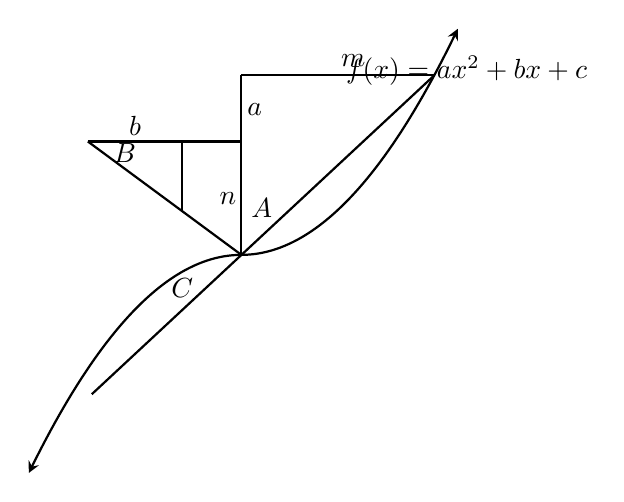
\begin{tikzpicture}[x=1cm, y=1cm, >=stealth]
  % Parabola: parabola_main
  \draw[<->, thick] plot[domain=-2.7:2.75, samples=100] (\x, {0.38*\x^2 + 0.0*\x + 0.0});
  % Segment: secant_line
  \draw[thick] (-1.90, -1.77) -- (2.45, 2.28);
  % Segment: vertical_stem
  \draw[thick] (0.00, 2.28) -- (0.00, -0.00);
  % Segment: top_horizontal_m
  \draw[thick] (0.00, 2.28) -- (2.45, 2.28);
  % Segment: left_horizontal_b
  \draw[thick] (-1.95, 1.44) -- (0.00, 1.44);
  % Segment: left_chord
  \draw[thick] (-1.95, 1.44) -- (0.00, -0.00);
  % Segment: left_drop
  \draw[thick] (-0.75, 1.44) -- (-0.75, 0.56);
  % Right Angle Marker: ra_top
  % Vertex at (0.00, 2.28)
  % Right Angle Marker: ra_left
  % Vertex at (-0.75, 1.44)
  \node at (2.86, 2.34) {$f(x) = ax^2 + bx + c$};
  \node at (1.42, 2.47) {$m$};
  \node at (0.17, 1.84) {$a$};
  \node at (-1.35, 1.64) {$b$};
  \node at (-0.17, 0.72) {$n$};
  \node at (0.26, 0.60) {$A$};
  \node at (-1.48, 1.29) {$B$};
  \node at (-0.75, -0.42) {$C$};
\end{tikzpicture}